%%
%% Commands for TeXCount
%TC:macro \cite [option:text,text]
%TC:macro \citep [option:text,text]
%TC:macro \citet [option:text,text]
%TC:envir table 0 1
%TC:envir table* 0 1
%TC:envir tabular [ignore] word
%TC:envir displaymath 0 word
%TC:envir math 0 word
%TC:envir comment 0 0
%%
%% For submission and review of your manuscript please change the
%% command to \documentclass[manuscript, screen, review]{acmart}.
%%
%% When submitting camera ready or to TAPS, please change the command
%% to \documentclass[sigconf]{acmart}.
%%
\documentclass[sigconf,authordraft, anonymous]{acmart}

\AtBeginDocument{%
  \providecommand\BibTeX{{Bib\TeX}}}

%% Rights management information.
%% Update these with your actual rights form values.
\setcopyright{acmlicensed}
\copyrightyear{2026}
\acmYear{2026}
\acmDOI{XXXXXXX.XXXXXXX}
\acmConference[ICCAD '26]{International Conference on Computer-Aided Design}{November 8--12, 2026}{San Jose, California, USA}
\acmISBN{978-1-4503-XXXX-X/2025/00}

%% Remove the copyright statement and ACM reference block from the PDF
\settopmatter{printacmref=false}
\renewcommand\footnotetextcopyrightpermission[1]{}
\pagestyle{plain}

\raggedbottom
\usepackage{lipsum}
\usepackage{wasysym} 
\usepackage{booktabs}
\usepackage{makecell}
\usepackage{svg}

%%
%% Author information
%%
\begin{document}

\title{TensorLift: Automatic Extraction of Tensor-Level ISA Semantics from Accelerator RTL via MLIR Semantic Lifting}

\author{Ruijie Gao}
\email{ruijieg@umich.edu}
\affiliation{%
  \institution{University of Michigan}
  \city{Ann Arbor}
  \state{Michigan}
  \country{United State of America}
}

\renewcommand{\shortauthors}{Gao et al.}

\begin{abstract}

Numerous tensor accelerator designs exist in academia and industry, yet most lack well-documented ISAs and the software tooling needed to use them, leaving fabricated silicon underutilized. Recent work (e.g., TAIDL and the ACT ecosystem) has shown that given a tensor-level ISA specification, complete software stacks including test oracles and compiler backends can be automatically generated. However, writing such specifications remains a manual, expert-driven process.

We present TensorLift, a fully automated framework that extracts tensor-level ISA specifications directly from accelerator RTL. Building on prior architecture-level model extraction that produces bit-level LLVM IR, TensorLift introduces an 8-pass MLIR semantic lifting pipeline that progressively recovers high-level tensor structure, including MAC idioms, saturation semantics, multi-dimensional buffer organizations, and data layout transformations. The pipeline emits specifications in the TAIDL formalism, immediately enabling automatic software stack generation through the ACT ecosystem.

We evaluate TensorLift on Gemmini, a systolic-array accelerator, extracting all 11 hardware instructions with a 97.5\% MLIR reduction. TensorLift discovers hardware features omitted from the hand-written reference, including pooling engine semantics and im2col hardware support. Correctness is validated through SMT equivalence proofs and simulator testing. TensorLift closes the loop from RTL to full software stack without manual ISA documentation.
\end{abstract}

% \begin{CCSXML}
% <ccs2012>
%  <concept>
%   <concept_id>00000000.0000000.0000000</concept_id>
%   <concept_desc>Replace with correct CCS terms</concept_desc>
%   <concept_significance>500</concept_significance>
%  </concept>
% </ccs2012>
% \end{CCSXML}

% \ccsdesc[500]{Replace with correct CCS terms}

\keywords{Tensor Accelerators, ISA Extraction, RTL Abstraction, MLIR, Semantic Lifting, Hardware-Software Interface}

\maketitle


\section{Introduction}
\label{sec:introduction}

\begin{figure}[t]
  \centering
  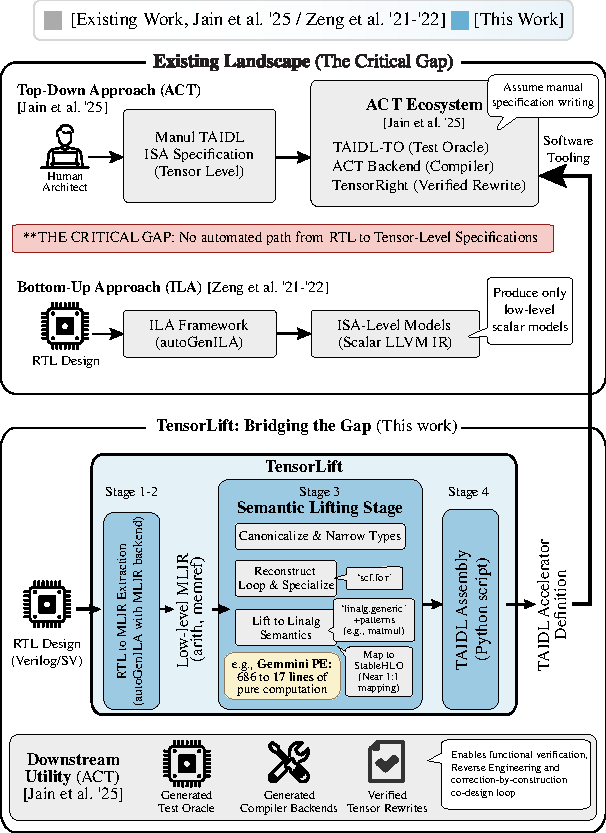
\includegraphics[width=\linewidth]{fig/overview.pdf}
  \caption{Overview of the existing landscape and TensorLift's role.
  The top-down ACT ecosystem~\cite{act-arxiv} assumes a manually written
  TAIDL specification, while the bottom-up ILA
  framework~\cite{autogeniladate, autogenilaiccad} produces only scalar-level models.
  TensorLift bridges this gap with an MLIR-based semantic lifting
  pipeline that automatically extracts tensor-level ISA semantics
  from RTL, enabling the full automated path from hardware design
  to ML framework integration.}
  \label{fig:overview}
\end{figure}

The rapid growth of deep learning workloads has driven a proliferation of specialized tensor accelerators in both academia and industry. Designs such as Gemmini, MAERI, SIGMA, Eyeriss, NVDLA, and FEATHER explore diverse microarchitectural innovations—systolic arrays, reconfigurable interconnects, flexible dataflow engines—to deliver orders-of-magnitude improvements in performance and energy efficiency over general-purpose processors. Meanwhile, a small number of platforms backed by major vendors, notably Google's TPU with XLA, Intel AMX with oneDNN, and NVIDIA GPUs with CUDA/cuDNN, enjoy mature compiler toolchains that connect them seamlessly to frameworks like PyTorch, JAX, and TensorFlow. The contrast is stark: as Table~\ref{tab:accel-landscape} summarizes, accelerators with mature, end-to-end compiler support number fewer than five, while over a dozen open-source designs lack any usable compiler backend. These accelerators can only be exercised through hand-written kernel libraries that cover a narrow set of operators and miss cross-layer fusion opportunities, leaving the vast majority of proposed hardware unable to run real ML models end-to-end.

\begin{table}[t]
  \centering
  \scriptsize
  \caption{Software stack readiness of representative open-source tensor/DNN accelerators.
  \CIRCLE{} = available, \LEFTcircle{} = partial/limited, \Circle{} = unavailable.
  \textbf{TensorLift} targets accelerators with open RTL (\CIRCLE{}/\LEFTcircle{} in col.~3)
  but missing ISA specifications (\Circle{} in col.~1).}
  \label{tab:accel-landscape}
  \setlength{\tabcolsep}{3pt}
  \begin{tabular*}{\linewidth}{@{\extracolsep{\fill}}lcccc@{}}
    \toprule
    Accelerator
      & \makecell{ISA\\Spec}
      & \makecell{Compiler\\Backend}
      & \makecell{Open\\RTL}
      & \makecell{Test\\Oracle} \\
    \midrule
    % --- No compiler backend ---
    MAERI~\cite{maeri-asplos2018}
      & \Circle      & \Circle      & \CIRCLE      & \Circle \\
    SIGMA~\cite{sigma-hpca2020}
      & \Circle      & \Circle      & \CIRCLE      & \Circle \\
    Eyeriss~\cite{eyeriss-jssc2017}
      & \Circle      & \Circle      & \LEFTcircle  & \Circle \\
    MAGNet~\cite{venkatesan2019magnet}
      & \Circle      & \Circle      & \CIRCLE      & \Circle \\
    DNNBuilder~\cite{dnnbuilder-iccad2018}
      & \Circle      & \Circle      & \CIRCLE      & \Circle \\
    FlexASR~\cite{flexasr}
      & \Circle      & \Circle      & \CIRCLE      & \Circle \\
    SPAGHETTI~\cite{spaghetti}
      & \Circle      & \Circle      & \CIRCLE      & \Circle \\
    \midrule
    % --- Partial compiler support ---
    NVDLA~\cite{nvdla}
      & \LEFTcircle  & \LEFTcircle  & \CIRCLE      & \LEFTcircle \\
    Gemmini~\cite{gemmini-dac2021}
      & \LEFTcircle  & \LEFTcircle  & \CIRCLE      & \LEFTcircle \\
    VTA~\cite{vta}
      & \LEFTcircle  & \LEFTcircle  & \CIRCLE      & \LEFTcircle \\
    DnnWeaver~\cite{dnnweaver-micro2016}
      & \Circle      & \LEFTcircle  & \CIRCLE      & \Circle \\
    \midrule
    % --- Mature (baselines) ---
    Google TPU~\cite{tpuv1}
      & \CIRCLE      & \CIRCLE      & \Circle      & \CIRCLE \\
    Intel AMX~\cite{amx}
      & \CIRCLE      & \CIRCLE      & \Circle      & \CIRCLE \\
    \bottomrule
  \end{tabular*}
\end{table}

The root cause of this software deficit lies upstream of the compiler: the ISA semantics of most accelerators have never been formally defined. In the CPU world, the ISA serves as the foundational contract between hardware and software—compilers, simulators, and verification tools are all built on top of it. For accelerators, however, ISA information is typically scattered across RTL source code, informal documentation, or exists only in the minds of hardware designers. Huang et al. formalized this observation with the Instruction-Level Abstraction (ILA), noting that the accelerator community lacks both a common framework for specifying accelerator behavior and a unified way to reason about programs that interact with accelerators. From the programming language side, Exo demonstrated that proprietary hardware interfaces force each company to maintain its own compiler fork—a cost that discourages hardware innovation and entrenches legacy platforms whose dominance stems from ecosystem lock-in rather than architectural merit. Figure~\ref{fig:overview} summarizes this landscape: the top-down ACT ecosystem assumes a hand-written TAIDL specification, while the bottom-up ILA framework produces only scalar-level models, leaving no automated path from RTL to tensor-level semantics.

Recent work has made significant strides in closing the gap from ISA specification downward. TAIDL, presented at MICRO 2025, introduced the first domain-specific language for defining tensor accelerator ISAs and showed how test oracles can be auto-generated from these definitions, achieving orders-of-magnitude speedups over hand-crafted functional simulators like Gemmini Spike. Building on TAIDL, the ACT project demonstrated that sound and complete compiler backends can be automatically generated from ISA descriptions alone, producing code that matches or outperforms hand-optimized kernel libraries. Together, these efforts establish a compelling pipeline from ISA specification to ML framework integration: given a TAIDL definition, ACT generates a compiler backend that plugs into XLA, enabling end-to-end execution from JAX or PyTorch. However, this pipeline has a critical prerequisite: someone must first write the TAIDL specification by hand—a process that requires deep understanding of the accelerator's architectural state, instruction encoding, and tensor-level semantics.

This manual specification bottleneck creates a broken pipeline in practice. On the hardware side, RTL designs iterate rapidly as architects explore microarchitectural trade-offs; on the software side, TAIDL and ACT can automate everything downstream of the ISA spec but cannot function without one. The result is that building compiler and simulator support still involves considerable manual effort, slowing innovation and widening the gap between hardware and software research communities. The 3LA methodology corroborates this assessment: even with the ILA formal framework available, testing prototype accelerator designs on real applications end-to-end remains prohibitively difficult due to the cost of constructing specialized compiler and simulator support. This bottleneck also limits the potential of emerging LLM-based agents for EDA, which are poised to transform hardware design workflows but require machine-readable hardware semantics as input—semantics that, for most accelerators, simply do not exist in any structured form.

In this paper, we present TensorLift, the first approach to automatically extract tensor-level ISA semantics from accelerator RTL. TensorLift employs an MLIR-based semantic lifting pipeline consisting of seven progressive passes that transform low-level CIRCT/FIRRTL representations into high-level tensor operations, bridging the abstraction gap between gate-level hardware and the ISA-level semantics required by tools like TAIDL and ACT. We evaluate TensorLift on the Gemmini accelerator, achieving 100\% instruction coverage by extracting all 11 hardware instructions. Our analysis also reveals that 4 of the 15 entries in TAIDL's Gemmini specification—softmax, GELU, layernorm, and fused add-with-transpose—are in fact software-composed macro-instruction sequences rather than hardware ISA primitives, a distinction that TensorLift's bottom-up extraction naturally surfaces. By filling the frontmost gap in the RTL-to-framework pipeline, TensorLift enables a fully automated path from RTL to ML framework integration, as illustrated in Figure~\ref{fig:overview}. The complete pipeline---RTL through TensorLift to ISA specification, then through ACT to a compiler backend plugged into XLA---requires no manual specification effort at any stage.

In summary, this paper makes the following contributions:

\begin{itemize}
\item We propose the first method for automatically extracting tensor-level ISA semantics from accelerator RTL, eliminating the manual specification bottleneck that currently blocks the adoption of automated compiler generation tools.
\item We design a 8-pass MLIR-based semantic lifting pipeline that progressively abstracts from CIRCT/FIRRTL through control flow recovery, memory access pattern analysis, and datapath semantics extraction to tensor-level operation identification.
\item We evaluate TensorLift on the Gemmini accelerator, demonstrating 100\% hardware instruction coverage (11/11) and identifying the boundary between true hardware ISA and software-composed macro-instructions.
\item We complete the end-to-end automated pipeline from RTL to ML framework, enabling agile software stack construction that can keep pace with hardware design iteration.
\end{itemize}





\section{Background}
\label{sec:background}

% TODO: Write background


\subsection{Hardware-Software Interfaces in Tensor Accelerators}
\label{subsec:hw-sw-interface}

Tensor accelerators occupy a fundamentally different point in the design space than scalar or vector processors.
Rather than executing fine-grained instruction streams over flat register files and cache-coherent memory, they expose \emph{coarse-grained} operations that consume and produce multi-dimensional tensors and replace implicit caches with \emph{explicitly managed} on-chip memories (scratchpads, accumulator banks).
Gemmini~\cite{gemmini-dac2021}, Berkeley's open-source systolic-array generator, is representative: it attaches to a Rocket core as a RoCC accelerator~\cite{chipyard} with non-standard RISC-V custom instructions, and its programmer-visible state consists of a row-addressed scratchpad and an accumulator.
Its ISA exposes only configuration, DMA data-movement, and matrix-multiply execution instructions---every operation simultaneously specifies \emph{what} to compute, \emph{where} operands live in a private memory hierarchy, and \emph{how} data should be staged.

This distinctiveness places heavy demands on compiler infrastructure.
ML frameworks feed tensor IR (StableHLO, Linalg, TOSA) into backends such as XLA~\cite{xla}, TVM~\cite{tvm}, or IREE~\cite{iree}, which must lower high-level operations to the accelerator's native instructions.
Doing so correctly requires tiling and fusing loop nests to fit scratchpad capacity, scheduling explicit DMA transfers, allocating scratchpad regions, and orchestrating double-buffering---all of which presuppose a precise model of what each instruction does to which piece of tensor state.

Consider lowering a single XLA \texttt{dot} $C{=}A{\cdot}B$ for matrices exceeding Gemmini's $16{\times}16$ tile.
The backend must emit a tiled sequence: \texttt{config\_ex}/\texttt{config\_ld}/\texttt{config\_st} to set dataflow and stride parameters; \texttt{mvin}/\texttt{mvin2} to stage tiles of $A$ and $B$ into the scratchpad; \texttt{preload} followed by \texttt{compute\_preloaded} (or \texttt{compute\_accumulated}) to fire the systolic array for each output tile; and \texttt{mvout} to drain results.
Generating this sequence requires the backend to know, for every instruction, which tensor tile it touches, which scratchpad region it occupies, and how its output composes with subsequent operations.

This is precisely where most accelerators fall short.
Mapping tensor IR to an instruction sequence presupposes a \emph{machine-readable} ISA that specifies both the binary encoding and the \emph{tensor-level semantics} of each instruction.
For Gemmini, semantics live informally in prose documentation, the Chisel RTL, and a hand-written Spike functional model; most open-source accelerators offer only RTL and perhaps a driver.
Building a backend today is therefore largely an exercise in \emph{manual reverse-engineering of the RTL}---a human infers what each custom instruction means at the tensor level and re-encodes that knowledge by hand.
This is the bottleneck that motivates automatically lifting tensor-level ISA semantics directly from RTL.

\subsection{Automated Compiler Generation and the Specification Bottleneck}


\subsection{RTL Extraction and MLIR-Based Semantic Lifting}

\section{TensorLift Pipeline}
\label{sec:pipeline}

Figure~\ref{fig:overview} (lower half) decomposes TensorLift into three sequential stages that, taken together, transform an unannotated RTL design into a TAIDL specification consumable by the ACT ecosystem.
\textbf{Stage~1 (RTL-to-MLIR extraction, \S\ref{subsec:stage1})} uses an extended autoGenILA backend to symbolically unroll the design and emit, for every (instruction, ASV) pair, a low-level MLIR function written in the \texttt{arith}, \texttt{memref}, \texttt{scf}, and \texttt{affine} dialects.
\textbf{Stage~2 (semantic lifting, \S\ref{subsec:stage2})} runs an eight-pass MLIR rewrite pipeline that progressively normalizes bit-manipulation idioms, recovers multiply--accumulate and saturation structure, specializes control modes, reconstructs MAC chains as \texttt{scf.for} reductions, and lifts dot-product loops into the \texttt{linalg} dialect; a final metadata-emission pass annotates the lifted MLIR with structured \texttt{taidl.*} attributes.
\textbf{Stage~3 (TAIDL assembly, \S\ref{subsec:stage3})} consumes those annotations through a generic Python emitter that materializes a TAIDL specification with XLA-HLO-style semantics, together with the data-model declarations and instruction encodings.
The boundaries between stages are deliberately deep: Stage~1 owns all hardware-level reasoning and produces a behavior-equivalent yet still-bit-level model; Stage~2 owns all rewriting from bit-level to tensor-level semantics and is purely an MLIR pass pipeline; Stage~3 is a syntactic projection into the surface TAIDL language.
The remainder of this section walks through each stage in turn.

\subsection{Stage 1: RTL-to-MLIR Extraction}
\label{subsec:stage1}

TensorLift's first stage builds on autoGenILA~\cite{autogenilaiccad,autogeniladate}, a two-pass framework for recovering instruction-level behavior from synthesizable RTL.
Given a flattened Verilog design and a small per-instruction harness file that pins control inputs to a particular opcode while leaving data inputs symbolic, autoGenILA first uses path-sensitive taint analysis~\cite{autogenilaiccad} to identify the subset of registers that are \emph{architectural state variables} (ASVs)---registers whose values persist across instruction boundaries and form the programmer-visible state.
It then processes one (instruction, ASV) pair at a time~\cite{autogeniladate}: it symbolically unrolls the design over a user-supplied cycle bound, walks the resulting AST and constraint DAG with handlers for arithmetic, comparison, ITE/case mux, bit-select, concatenation, and submodule-call constructs, and emits an LLVM IR function whose arguments are the instruction inputs and current ASV values, and whose return value is the next-state value of the chosen ASV.
Together, the two passes yield a per-instruction architectural model that is bit-equivalent to the RTL by construction, no longer dependent on simulator infrastructure, and amenable to formal reasoning.

Although autoGenILA is the right starting point---it solves the \emph{extraction} problem with provable bit-equivalence---its output is unsuitable for tensor-level reasoning in two ways.
First, the LLVM IR backend is structurally tuned for compiled execution: it lowers conditional updates into branches and \texttt{phi} nodes, replaces typed memory accesses with pointer arithmetic, and---most consequentially---discards the RTL signal-name provenance that downstream lifting passes need to recognize buffers semantically (``which scalar argument carries the activation tile, and which carries the accumulator?'').
Second, autoGenILA was designed and evaluated on scalar RISC-V cores, and several construct families that arise routinely in DNN accelerators---signed division and modulo for DMA address arithmetic, and update functions whose intermediate constraint width does not match the declared return width---either trip the constraint dispatcher or produce verifier-rejected IR.
Both shortcomings have to be repaired before semantic lifting can proceed.

\paragraph{TensorLift's modifications.}
We retain autoGenILA's taint-based ASV inference, symbolic unrolling, and constraint-DAG traversal entirely; the modifications consist of a new code generator that replaces the LLVM IR backend, plus a small automation layer wrapped around the extraction. The original LLVM IR backend remains available unchanged and is reused as a verification oracle (\S\ref{sec:evaluation}). Concretely, the changes are:

\begin{enumerate}
\item \textbf{An MLIR-producing update-function backend.}
We add an alternative backend, \texttt{MLIRUpdateFunctionGen}, that mirrors autoGenILA's existing constraint-handler dispatch---two-operand and one-operand arithmetic, ITE/case/switch mux, bit-select and concatenation, dynamic memory selection, and submodule-call constructs---but emits MLIR in the \texttt{arith}, \texttt{memref}, \texttt{scf}, and \texttt{affine} dialects rather than LLVM IR.
The choice of MLIR is not cosmetic: the \texttt{scf} dialect preserves \texttt{if}/\texttt{else} regions instead of branching, \texttt{memref} preserves indexed loads and stores instead of pointer arithmetic, and the dialect-aware rewrite framework~\cite{mlir-cgo2021,mlir-pattern-rewriting} underpins every pass in Stage~2 (\S\ref{subsec:stage2}).
The backend is selected by a single CLI flag, shares all of autoGenILA's parsing, taint, and traversal infrastructure unchanged, and every emitted file is round-tripped through \texttt{mlir-opt} as a sanity check before lifting.

\item \textbf{Time-indexed input memrefs.}
The natural translation of autoGenILA's input model would lower each module input signal at each unroll cycle as an independent scalar argument, so a 36-cycle unroll of a controller with eleven inputs would produce nearly four hundred unrelated scalars.
Our backend instead packs the time series of each input into a single \texttt{memref}-typed argument whose leading dimension is the unroll bound and whose element type is the original signal width, with one explicit \texttt{memref.load} per cycle inside the function body.
This grouping carries no semantic content of its own, but it is what later allows the loop-reconstruction pass to recognize MAC chains as indexable reductions and lift them into \texttt{scf.for} loops (\S\ref{subsec:stage2}); without the grouping, the same chain decomposes into hundreds of unrelated scalars and is unrecoverable.

\item \textbf{RTL signal-name provenance via the \texttt{taidl.arg\_names} attribute.}
For each emitted \texttt{func.func}, the backend attaches the ordered list of original RTL signal names (\texttt{io\_in\_a\_0}, \texttt{io\_srams\_read\_0\_resp\_bits\_data}, $\ldots$) as an \texttt{ArrayAttr} on the function operation.
The lifting passes downstream consult this attribute to classify arguments as data buffers, control attributes, or accumulator state, and the TAIDL assembler in Stage~3 uses the same attribute to derive instruction-operand names matching the convention used by hand-written TAIDL specifications~\cite{taidl-ae-micro2025}.
Without this hook, every shred of semantic information about RTL signals would be lost the moment the constraint DAG is lowered into anonymous MLIR \texttt{Value}s.

\item \textbf{Robustness fixes for accelerator construct families.}
Two construct families absent from autoGenILA's published evaluation but ubiquitous in DNN accelerators required completing the dispatcher.
The first is signed and unsigned division and modulo, which appear in the DMA stride and pixel-repeat address arithmetic of Gemmini's load and store controllers; we add the corresponding \texttt{arith.divsi}/\texttt{remsi} (and unsigned-variant) cases to the constraint handler.
The second is constraint expressions whose inferred intermediate width exceeds the declared return width of an update function---a common situation when a width-conservative \texttt{i32} traversal ultimately writes a one-bit predicate register; we insert an explicit \texttt{trunci}/\texttt{extui} adapter at the function return so the emitted MLIR satisfies the verifier under all combinations of intermediate and declared widths.

\item \textbf{An automation harness around the extraction.}
Vanilla autoGenILA expects the user to hand-author four ancillary files per design---a Yosys flatten script, a reset script, a per-instruction harness (\texttt{instr.txt}), and an ASV target list (\texttt{allowed\_target.txt})---together with knowledge of clock and reset signal names, pipeline depths, and per-opcode control vectors.
We replace this with a small set of generators that, given only a directory of SystemVerilog files and a top-module name, automatically (a)~run Yosys with FIRRTL-aware assertion stripping (\texttt{chformal -remove}, required because Chisel \texttt{assert} calls survive into the synthesized netlist) and post-process its output to satisfy autoGenILA's parser, (b)~enumerate ASV targets by walking flip-flop declarations and grouping vector slices, and (c)~discover instruction encodings from the RTL decoder for funct-field ISAs.
The harness reduces the per-design manual input to two items, an RTL directory and a top-module name, which is what makes the end-to-end pipeline of Figure~\ref{fig:overview} viable in practice.
\end{enumerate}

The result of Stage~1 is a corpus of MLIR files, one per (instruction, ASV) pair, each containing a single \texttt{func.func} carrying the \texttt{taidl.arg\_names} attribute, written entirely in the \texttt{arith}, \texttt{memref}, \texttt{scf}, and \texttt{affine} dialects, and provably equivalent (modulo the LLVM IR equivalence proofs of \S\ref{sec:evaluation}) to autoGenILA's bit-accurate model of the RTL.
As Figure~\ref{fig:code} (middle panel) illustrates, even a single Gemmini PE produces 686 lines of MLIR at this stage---an artifact of the bit-level structure of autoGenILA's traversal, in which the core multiply--accumulate is buried under 383 sign-extension and bit-packing operations.
Recovering tensor-level structure from this representation is the job of Stage~2.

\subsection{Stage 2: Semantic Lifting}
\label{subsec:stage2}

Stage~2 is the analytical core of TensorLift: an eight-pass MLIR pipeline, registered behind a single \texttt{tensorlift-opt} tool, that turns the bit-accurate Stage~1 output into MLIR whose structure mirrors tensor-level semantics. The passes fall into four phases (2\,+\,3\,+\,2\,+\,1 passes respectively): (\textbf{A}) bit-manipulation canonicalization, (\textbf{B}) idiom detection for MAC, control-mode, and saturation patterns, (\textbf{C}) loop and tensor-shape reconstruction, and (\textbf{D}) TAIDL metadata emission. Table~\ref{tab:lifting-passes} lists the eight passes; the remainder of this subsection highlights the design choices that distinguish the pipeline from a conventional MLIR lowering.

\begin{table}[t]
\centering
\caption{TensorLift's eight-pass MLIR semantic-lifting pipeline. Each pass is named with its \texttt{tensorlift-opt} flag.}
\label{tab:lifting-passes}
\setlength{\tabcolsep}{3pt}
\renewcommand{\arraystretch}{1.18}
\scriptsize
\begin{tabular}{@{}l p{5.9cm}@{}}
\toprule
Phase / Pass & What it does \\
\midrule
A1 \texttt{canon-bitmanip}
& Collapses the bit-by-bit sign-extension chains that autoGenILA emits when traversing Verilog \texttt{\$signed} contexts into a single \texttt{arith.extsi}; the dominant source of code reduction on PEs. \\
A2 \texttt{narrow-types}
& Folds redundant \texttt{trunci}/\texttt{ext} round trips left over after canonicalization, while deliberately preserving the \texttt{extsi(trunci(\,))} idioms that Pass~B5 must recover as saturation. \\
\addlinespace[1pt]
B3 \texttt{detect-mac}
& Walks each \texttt{addi} back through width casts to find a multiplier and recovers its pre-extension inputs; tags the pair with \texttt{tensorlift.mac} when the operand widths are hardware-realistic, filtering out bit-packing artifacts. \\
B4 \texttt{specialize-control}
& Constant-folds the loads of the fixed control inputs of the instruction under analysis (taken from the same \texttt{instr.txt} that drove Stage~1), letting downstream canonicalization eliminate the \texttt{select} chains that selected between hardware modes. \\
B5 \texttt{detect-clamp}
& Recognizes the hardware fixed-point saturation idiom \texttt{ext(trunci(x))} and annotates the surviving extension with the recovered clamp range and signedness. \\
\addlinespace[1pt]
C6 \texttt{reconstruct-loops}
& Builds a use--def chain over MAC-annotated additions whose accumulator input is the previous MAC's output, and---for chains of length~$\geq\!2$---materializes the chain as an \texttt{scf.for} reduction with a single \texttt{iter\_arg}. \\
C7 \texttt{lift-to-linalg}
& Verifies that a reconstructed \texttt{scf.for} matches the canonical dot-product shape (single \texttt{iter\_arg}, two memref loads at the induction variable, multiply--add--yield) and tags it with \texttt{linalg\_op = "dot\_product"}. \\
\addlinespace[1pt]
D8 \texttt{emit-taidl-metadata}
& Walks the lifted module to classify each \texttt{memref} argument by its load/store footprint, label scalar arguments as control attributes, infer grid dimensions from coordinate suffixes in target ASV names, and emit a closed set of \texttt{taidl.*} attributes consumed by Stage~3. \\
\bottomrule
\end{tabular}
\end{table}

\paragraph{Annotation-driven, accelerator-agnostic.}
With the sole exception of loop reconstruction (C6), Phases~B--D do not rewrite the IR but instead attach \texttt{tensorlift.*} attributes to existing operations; the next pass keys off those attributes.
This decoupling lets each pass be verified independently against MLIR's verifier and against the LLVM IR oracle (\S\ref{sec:evaluation}), and lets unrecognized dataflow degrade gracefully: an instruction whose body fails to match the MAC or clamp template simply does not receive the corresponding annotation, and the Stage~3 assembler falls back to an opaque \texttt{copy} or \texttt{unknown} semantics rather than producing incorrect TAIDL.
None of the eight passes contains any Gemmini- or VTA-specific identifier: the structural cues they rely on (sign-extension chains, MAC fan-in, fixed-point clamp idioms, accumulator def-use chains, dot-product loop shape, and RTL signal-name suffixes such as \texttt{pool\_*} or \texttt{im2col\_*}) are properties of common synthesizable RTL patterns rather than of any particular ISA.
The only per-instruction input is the control vector consumed by Pass~B4, which is itself derived automatically (\S\ref{subsec:stage1}); the same \texttt{tensorlift-opt} binary lifts Gemmini's PE, its DMA controllers, and VTA's TensorGemm and TensorAlu without modification.

On the running example, the eight passes together reduce the Gemmini PE update function from 686 lines of bit-level MLIR to 49 lines, of which only 17 encode the actual computation core \texttt{clamp(dot(\%A,\%B)+\%C)}; the remaining lines are arguments, loads, stores, and the \texttt{taidl.*} metadata that Stage~3 turns into a TAIDL specification (\S\ref{sec:evaluation}).

\subsection{Stage 3: TAIDL Assembly}
\label{subsec:stage3}

Stage~3 is a generic Python emitter that turns the artifacts of Stage~2 into a complete TAIDL specification of the form shown in Listing~\ref{lst:taidl-example}.
It consumes two parallel inputs: the \texttt{taidl.*}-annotated MLIR produced by Pass~D8, and a \texttt{state\_machine.json} file produced by an auxiliary script that reads autoGenILA's per-ASV LLVM IR independently of the lifting pipeline.
Both inputs are derived automatically from Stage~1's output; Stage~3 itself contains no per-accelerator code paths.

\paragraph{Assembling the tensor semantics.}
The assembler operates on a closed vocabulary of thirteen \texttt{taidl.*} attribute keys.
After parsing each annotated function into a Python record, it groups buffers across all functions by the triple \emph{(category, type, width)} to derive one \texttt{add\_data\_model} declaration per signature, then merges the per-(instruction, ASV) functions emitted by Stage~1 back into per-instruction groups via a four-level priority chain---an explicit \texttt{--instr-names} list, the original \texttt{instr.txt}, path-based discovery of \texttt{instr.txt} alongside the input MLIR, and finally a longest-prefix heuristic that requires at least three sibling names to commit a prefix---so the same code path handles Gemmini's four-instruction \texttt{ExecuteController} and VTA's single-instruction modules without modification.
Within each group it selects the metadata record with the richest dataflow as a template and dispatches its \texttt{tensor\_op} through a small table that maps each value to its XLA-HLO-style template: \texttt{mac}/\texttt{dot\_product} expand to \texttt{convert+dot+add} (with optional \texttt{clamp}), \texttt{pool} to \texttt{reduce(max)}, \texttt{im2col\_matmul} to \texttt{reshape+dot+add}, and \texttt{copy} to a buffer-to-buffer move.
A second sweep over indexed signal bases (\texttt{strides\_0/1/2}, \texttt{scales\_0/1/2}, $\ldots$) emits \texttt{IF/ELSE} bank-selection bodies for multi-bank configuration instructions, which is what allows TensorLift's specification to capture the three independently configurable DMA banks that the hand-written Gemmini TAIDL collapses into a single \texttt{@a.stride} parameter.
The output is a single Python file that calls the TAIDL API to register data models, instructions, semantics, and (when a state machine is available) initial states, constraints, and updates; adding a new tensor-op family requires extending only the dispatch table and the \texttt{taidl.tensor\_op} vocabulary in Pass~D8.

\paragraph{Inferring the instruction state machine.}
The constraints and updates that gate instructions---e.g., that \texttt{compute\_preloaded} can fire only after \texttt{preload} has armed the controller---are not visible in the Stage~2 output, which is per-instruction by construction.
We recover them with an auxiliary script that reads the same per-ASV update functions in their LLVM IR form, where the \texttt{icmp eq} comparisons against control registers that Pass~A1 collapses are still intact.
The script auto-detects the FSM register by scoring all multi-writer scalar ASVs against three predicates: small bit-width ($\leq\!8$), the presence of \texttt{icmp eq} comparisons \emph{at the register's own bit-width} (which filters out boolean event flags), and at least two distinct compared constants.
Once the FSM register is fixed, each instruction's constraint is the set of constants its update functions compare the register against, with pipeline-flush boundary values filtered as boilerplate; instructions that write the FSM but test no explicit value are handled by a binary-FSM complement rule, in which a writer of the inverse state is gated on the negation of the active state.
Updates are derived symmetrically from non-identity register writes: a write of an \texttt{rs1}/\texttt{rs2} command field into a configuration register becomes \texttt{@s.<reg> = @a.<reg>}, an FSM transition becomes \texttt{@s.<fsm> = <new\_state>}, and any write whose right-hand side is neither a constant nor a single instruction argument is dropped---its semantics already live in the tensor body emitted by the assembler.
The script writes \texttt{state\_machine.json}, which the assembler ingests in its final emission step.

On the running Gemmini ExecuteController example, this two-pronged Stage~3 reproduces the structure of the hand-written reference TAIDL specification: the four extracted instructions (\texttt{config\_ex}, \texttt{preload}, \texttt{compute\_preloaded}, \texttt{compute\_accumulated}) carry the same constraints and the same state-update relations as the reference, with the only difference being that the inferred FSM register is named \texttt{control\_state} (its RTL identifier) where the hand-written specification names it \texttt{preload} (a TAIDL source-level alias).
This is purely a name choice in the generated TAIDL source: as we report in \S\ref{sec:evaluation}, the test oracles produced from TensorLift's specification are character-identical to those produced from the hand-written reference, because the oracle generator alpha-renames state registers consistently across both inputs.
Together with Stages~1--2, the pipeline closes the loop from RTL to ACT-consumable TAIDL, replacing what is otherwise a hand-authoring step with a deterministic lifting and assembly process.

\section{Evaluation}
\label{sec:evaluation}

We evaluate TensorLift along four axes:
(\S\ref{subsec:lifting-effectiveness})~how effectively the lifting pipeline compresses bit-level MLIR into tensor-level semantics;
(\S\ref{subsec:correctness})~whether the lifted semantics are provably equivalent to the RTL;
(\S\ref{subsec:completeness})~how the automatically extracted specification compares to a hand-written reference; and
(\S\ref{subsec:e2e})~whether the extracted specification can drive end-to-end compiler backend generation.

\subsection{Experimental Setup}
\label{subsec:setup}

We target two open-source tensor accelerators.
\textbf{Gemmini}~\cite{gemmini-dac2021} is a systolic-array accelerator (16$\times$16, INT8 MAC) generated via the Chipyard~\cite{chipyard} SoC framework in the \texttt{GemminiRocketConfig} configuration.
It attaches to a Rocket core~\cite{asanovic2016rocket} as a RoCC coprocessor~\cite{chipyard} and exposes three hardware controllers (ExecuteController, LoadController, StoreController) with 11 hardware instructions across configuration, DMA data movement, and matrix execution.
\textbf{VTA}~\cite{vta} is TVM's Versatile Tensor Accelerator in the \texttt{DefaultDe10Config} configuration (16-element GEMM engine, ALU, INT8), with four datapath modules (TensorGemm, TensorAlu, Store, GenVMECmd).

All formal verification uses Z3~\cite{z3} bitvector SMT solving.
Cycle-level validation uses the Gemmini Spike functional simulator~\cite{gemmini-spike}.
The hand-written reference specification is the TAIDL MICRO~2025 artifact~\cite{taidl-ae-micro2025}.

\subsection{Semantic Lifting Effectiveness}
\label{subsec:lifting-effectiveness}

\begin{figure}[t]
  \centering
  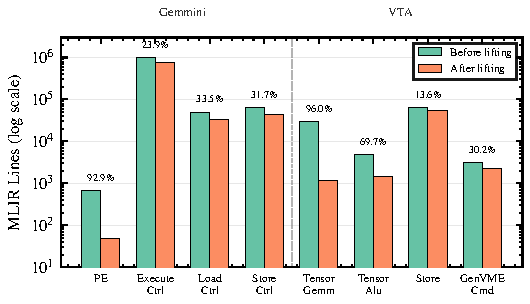
\includegraphics[width=\linewidth]{fig/lifting_results.pdf}
  \caption{MLIR line counts before and after TensorLift's 8-pass lifting pipeline, across all modules of Gemmini and VTA. Percentages indicate reduction. Compute-dominated modules (PE, TensorGemm) achieve the highest reduction because their bit-manipulation chains collapse under canonicalization, while DMA/control modules retain irreducible FSM and address logic.}
  \label{fig:lifting-results}
\end{figure}

\begin{table}[t]
\centering
\caption{Cross-accelerator lifting summary. ``Before'' and ``After'' report total MLIR lines across all per-(instruction, ASV) files in each module.}
\label{tab:lifting-summary}
\setlength{\tabcolsep}{3pt}
\scriptsize
\begin{tabular}{@{}ll r r r r@{}}
\toprule
Accelerator & Module & Files & Before & After & Reduction \\
\midrule
\multirow{4}{*}{Gemmini}
  & PE (TileWithReset) & 1    &     686 &      49 & \textbf{92.9\%} \\
  & ExecuteController  & 80   & 997{,}760 & 759{,}360 & 23.9\% \\
  & LoadController     & 23   &  50{,}004 &  33{,}244 & 33.5\% \\
  & StoreController    & 23   &  63{,}313 &  43{,}269 & 31.7\% \\
\cmidrule{2-6}
  & \textit{Total}     & \textit{127} & \textit{1{,}111{,}763} & \textit{835{,}922} & \textit{24.8\%} \\
\midrule
\multirow{4}{*}{VTA}
  & TensorGemm  &  9 & 29{,}745 &  1{,}183 & \textbf{96.0\%} \\
  & TensorAlu   & 10 &  4{,}832 &  1{,}465 & 69.7\% \\
  & Store       &  5 & 62{,}807 & 54{,}294 & 13.6\% \\
  & GenVMECmd   &  5 &  3{,}160 &  2{,}205 & 30.2\% \\
\cmidrule{2-6}
  & \textit{Total} & \textit{29} & \textit{100{,}544} & \textit{59{,}147} & \textit{41.2\%} \\
\midrule
\textbf{Combined} & & \textbf{156} & \textbf{1{,}212{,}307} & \textbf{895{,}069} & \textbf{26.2\%} \\
\bottomrule
\end{tabular}
\end{table}

Table~\ref{tab:lifting-summary} and Figure~\ref{fig:lifting-results} report the lifting results across all modules of both accelerators.
In total, TensorLift processes 156 MLIR files comprising 1{,}212{,}307 lines of bit-level MLIR, reducing them to 895{,}069 lines (26.2\% overall reduction).

The reduction varies dramatically with module function.
\textbf{Compute-dominated modules} achieve the highest compression.
The Gemmini PE collapses from 686 to 49 lines (92.9\%), with its computation core reduced to just 17 lines encoding \texttt{clamp(dot(\%A,\%B)+\%C)}---383 bit-by-bit sign-extension operations generated by Verilog \texttt{\$signed} contexts collapse to single \texttt{arith.extsi} casts under Phase~A canonicalization.
VTA's TensorGemm shows an even more dramatic pattern: MAC register targets shrink from 3{,}156 to 8 lines each (99.7\%), and the module overall reduces from 29{,}745 to 1{,}183 lines (96.0\%).

\textbf{Control-heavy modules} show moderate reduction (30--35\%).
Gemmini's LoadController (33.5\%) and StoreController (31.7\%) retain address computation, FSM transitions, and instruction muxing that cannot be simplified further---this is irreducible control logic.
VTA's TensorAlu (69.7\%) falls in between: its ALU dispatch logic contains real opcode muxing across five operations (MIN, MAX, ADD, SHR, SHL), but also benefits from collapsing cast chains around each operation.

\textbf{DMA engines} show the lowest reduction.
VTA's Store module (13.6\%) and Gemmini's ExecuteController (23.9\%) are dominated by large instruction decoders, multi-level address computation, and deep control logic with minimal bit-manipulation to canonicalize.
VTA's overall higher reduction (41.2\% vs.\ 24.8\%) reflects the fact that its TensorGemm module dominates the total (29K lines reduced to 1.2K), whereas Gemmini's ExecuteController dominates its total (998K lines across 80 files for 4 instructions $\times$ 20 ASVs).

\subsection{Correctness Verification}
\label{subsec:correctness}

We verify that TensorLift's lifted semantics are equivalent to the bit-level scalar model from which they are derived.
Since autoGenILA's extraction is provably bit-equivalent to the RTL by construction~\cite{autogenilaiccad, autogeniladate}, establishing equivalence between the lifted MLIR and autoGenILA's output transitively proves: \textbf{RTL behavior $\equiv$ TensorLift semantics}.

\begin{table}[t]
\centering
\caption{Formal verification results. Each row is a Z3 bitvector SMT proof establishing equivalence between the lifted MLIR and the bit-level scalar model.}
\label{tab:formal-verification}
\setlength{\tabcolsep}{3pt}
\scriptsize
\begin{tabular}{@{}l l l l@{}}
\toprule
Accelerator & Proof Target & Method & Scope \\
\midrule
\multirow{3}{*}{Gemmini}
  & PE MAC semantics     & Z3 bitvector  & All $2^{60}$ inputs \\
  & WS dataflow mux      & Z3 SMT        & Control specialization \\
  & DMA copy semantics   & Z3 + arrays   & All addresses/values \\
\midrule
VTA & 13 datapath targets & Z3 bitvector  & 4 modules \\
\bottomrule
\end{tabular}
\end{table}

Table~\ref{tab:formal-verification} summarizes the proofs.
For Gemmini, we verify the PE's multiply-accumulate core (\texttt{sext(a*b + trunc(c))}) against autoGenILA's LLVM IR output using Z3 bitvector reasoning over all $2^{60}$ possible input combinations, proving universal equivalence rather than relying on test vectors.
The weight-stationary dataflow mux (control specialization, Pass~B4) and DMA copy semantics (including strided access patterns) are similarly verified.
For VTA, 13 targets across all four datapath modules (TensorGemm, TensorAlu, Store, GenVMECmd) are proven equivalent to the LLVM IR output, covering both compute and control semantics.
Additionally, the lifting pipeline reveals a structural symmetry: VTA's input and weight index generators produce identical 146-line MLIR after lifting, consistent with the symmetric roles of these buffers in the GEMM engine.

As an independent cross-check, we compare TensorLift's extracted VTA semantics against the ISA operational semantics documented in the VTA specification~\cite{vta} (\S6--9).
All extracted instruction behaviors---GEMM tensor contraction, ALU element-wise operations with five opcodes, Store DMA command generation, and Load burst addressing---align with the published specification, confirming that the lifting pipeline recovers the documented ISA semantics without access to the specification document.

\subsection{Specification Completeness}
\label{subsec:completeness}

TensorLift extracts TAIDL specifications for all hardware instructions decoded and executed by Gemmini's three controllers (ExecuteController, LoadController, StoreController).

\paragraph{Comparison with hand-written reference.}
We compare TensorLift's extracted specification against the TAIDL MICRO~2025 artifact~\cite{taidl-ae-micro2025}, which provides a hand-written Gemmini specification.
TensorLift captures strictly richer semantics in three areas:

\begin{itemize}
\item \textbf{Multi-bank DMA configuration.}
The hand-written reference models each DMA load variant (\texttt{mvin\_spad}, \texttt{mvin\_acc}, etc.) with a single \texttt{@a.stride} parameter, implicitly assuming all three load engines share one configuration.
In practice, Gemmini's LoadController maintains \emph{three independent banks}, each with its own \texttt{stride}, \texttt{scale}, \texttt{shrink}, \texttt{block\_stride}, and \texttt{pixel\_repeat} registers (5 parameters $\times$ 3 banks = 15 registers total), with the active bank selected by the \texttt{state\_id} field (\texttt{rs1[4:3]}) of the instruction encoding.
This means the hand-written TAIDL cannot correctly simulate programs that use \texttt{mvin} and \texttt{mvin2} with different strides simultaneously---a real use case in tiled matrix multiplication where the A-tile and B-tile load from DRAM with different access patterns.
TensorLift's per-ASV extraction sees all three banks automatically because autoGenILA traces every register independently, and the assembler groups them by their indexed base name (e.g., \texttt{strides\_0}, \texttt{strides\_1}, \texttt{strides\_2}).

\item \textbf{Pooling engine semantics.}
TensorLift extracts 12 pooling configuration registers from the StoreController (\texttt{pool\_size}, \texttt{pool\_stride}, \texttt{pool\_upad}, \texttt{pool\_lpad}, \texttt{pool\_orows}, \texttt{pool\_ocols}, etc.) and generates \texttt{reduce(max) + clamp} semantics.
The hand-written reference does not model the pooling engine.

\item \textbf{Im2col hardware support.}
TensorLift extracts 9 im2col output ports from the ExecuteController and generates \texttt{reshape + dot} semantics, capturing the hardware's ability to perform im2col transformation on-the-fly during convolution execution.
\end{itemize}

We note that the hand-written reference also includes four entries---\texttt{softmax}, \texttt{GELU}, \texttt{layernorm}, and fused add-with-transpose---that are \emph{not} hardware ISA primitives.
These are software-composed multi-instruction sequences that use the host CPU's FPU for operations such as \texttt{exp()} and \texttt{divide()}.
No Gemmini RTL modules implement these operations.
TensorLift correctly identifies this hardware/software boundary by extracting only instructions that correspond to actual RTL decoder entries.

A natural question is why we do not directly compare compiler backends generated from the two specifications.
The reason is that the TAIDL MICRO~2025 artifact targets a \emph{functional simulator}, not a compiler backend.
Its specification describes how individual hardware instructions move data between scratchpad and accumulator at per-tile (16$\times$16) granularity---exactly the level of detail a cycle-accurate or functional simulator needs to replay an instruction trace.
However, a compiler backend requires a different abstraction: per-\emph{kernel} granularity that maps an entire HLO \texttt{dot} or convolution onto the hardware.
The MICRO~2025 artifact's per-instruction patterns are too granular for ACT's instruction selection, which expects CISC-level macro-instructions (e.g., \texttt{loop\_ws} matching a whole matrix multiply, \texttt{loop\_conv\_ws} matching a whole convolution).
TensorLift's specification provides this macro-level abstraction (Stage~3, \S\ref{subsec:stage3}), enabling ACT to generate a functional compiler backend as evaluated in the next section.

\subsection{End-to-End Compiler Backend Generation}
\label{subsec:e2e}

\begin{figure}[t]
  \centering
  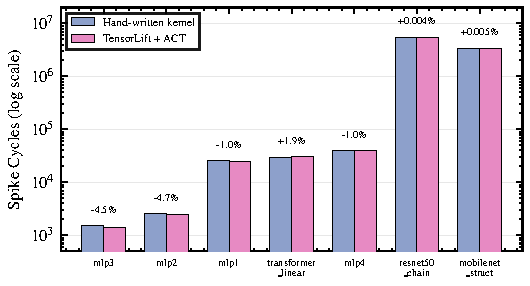
\includegraphics[width=\linewidth]{fig/latency_comparison.pdf}
  \caption{Cycle-level comparison on Gemmini's Spike simulator between hand-written kernels from gemmini-rocc-tests~\cite{gemmini-rocc-tests} and the automatically generated ACT compiler backend driven by TensorLift's extracted TAIDL specification. Labels show speedup (hand-written cycles\,/\,ACT cycles; ${>}\,1{\times}$ = ACT is faster). Geometric mean speedup is $1.014\times$.}
  \label{fig:latency}
\end{figure}

\begin{table}[t]
\centering
\caption{Latency comparison between hand-written Gemmini kernels and the TensorLift + ACT compiler backend, measured in Spike simulator cycles. Speedup $=$ hand-written\,/\,TensorLift+ACT (${>}\,1{\times}$ = ACT is faster). All benchmarks execute identical workloads (same layer shapes, dataflow, activation, scaling).}
\label{tab:latency}
\setlength{\tabcolsep}{3pt}
\scriptsize
\begin{tabular}{@{}l r r r@{}}
\toprule
Benchmark & Hand-written & TensorLift+ACT & Speedup \\
\midrule
mlp3               &       1{,}501 &       1{,}433 & $1.047\times$ \\
mlp2               &       2{,}571 &       2{,}451 & $1.049\times$ \\
mlp1               &      25{,}364 &      25{,}123 & $1.010\times$ \\
transformer\_linear &      29{,}732 &      30{,}302 & $0.981\times$ \\
mlp4               &      39{,}742 &      39{,}362 & $1.010\times$ \\
resnet50\_chain     &   5{,}544{,}077 &   5{,}544{,}303 & $1.000\times$ \\
mobilenet\_struct   &   3{,}408{,}414 &   3{,}408{,}581 & $1.000\times$ \\
\midrule
\multicolumn{3}{@{}l}{\textit{Geometric mean}} & $1.014\times$ \\
\bottomrule
\end{tabular}
\end{table}

To validate that TensorLift's extracted specification is sufficient for practical use, we feed it into the ACT compiler framework~\cite{act-arxiv} to automatically generate a Gemmini compiler backend, and compare the generated code against hand-written kernels on realistic workloads.

\paragraph{Methodology.}
We take TensorLift's extracted TAIDL specification and pass it to ACT, which generates an XLA-compatible compiler backend using equality saturation for instruction selection and constraint programming for scratchpad memory allocation.
Completing the path from specification to executable binary required engineering contributions to ACT: HLO frontend support for JAX-produced operations (e.g., \texttt{convolution}, \texttt{reduce\_max}), enode-level preconditions for correct convolution dispatch, and memory allocator support for multi-layer chains.
We then reimplement the benchmark suite from gemmini-rocc-tests~\cite{gemmini-rocc-tests}---the official bare-metal test suite provided by the Gemmini team---in JAX~\cite{jax2018github}, compiling through the ACT-generated backend.
For each benchmark, we compare the Spike cycle count of the ACT-compiled binary against the hand-written C kernel from gemmini-rocc-tests, ensuring identical workload parameters: layer shapes, weight-stationary dataflow, activation functions, scaling, and batch sizes.
The benchmark suite spans MLP, convolutional, and transformer workloads ranging from 2-layer networks (1{,}501 cycles) to full ResNet-50 (5{,}544{,}077 cycles) and MobileNet (3{,}408{,}414 cycles).

\paragraph{Results.}
Table~\ref{tab:latency} and Figure~\ref{fig:latency} report the results.
Across all seven benchmarks, the automatically generated backend achieves a geometric mean speedup of $1.014\times$ over hand-written kernels, with per-benchmark speedups ranging from $0.981\times$ to $1.049\times$.
The small MLP benchmarks (mlp2, mlp3) show the ACT backend running slightly faster ($1.047$--$1.049\times$), reflecting minor tiling differences in the generated code.
The transformer benchmark shows the only slowdown ($0.981\times$), attributable to per-tile configuration overhead in the generated instruction sequence.
On the large workloads that dominate real deployment---ResNet-50 (49 conv layers) and MobileNet (52 layers)---the speedup is $1.000\times$.

This result demonstrates that TensorLift, combined with ACT, enables a fully automated path from RTL to a functional, performance-competitive compiler backend.

\section{Related Work}
\label{sec:related}

% TODO: Write related work

\section{Conclusion}
\label{sec:conclusion}

% TODO: Write conclusion


\begin{acks}
% TODO: Add acknowledgments
\end{acks}

\clearpage

\bibliographystyle{ACM-Reference-Format}
\bibliography{references}

\end{document}
